\newpage
\subsection{Static verification of a bolted joint}
	
	\paragraph{Problem} Starting with the electric motor in figure \ref{ex:motorsketch} that transmits a nominal power $P = 8kW$ at an angular speed of $n = 750 rev/min$ to a belt drive with unit transmission ratio.
	\begin{figure}[b!]
		\centering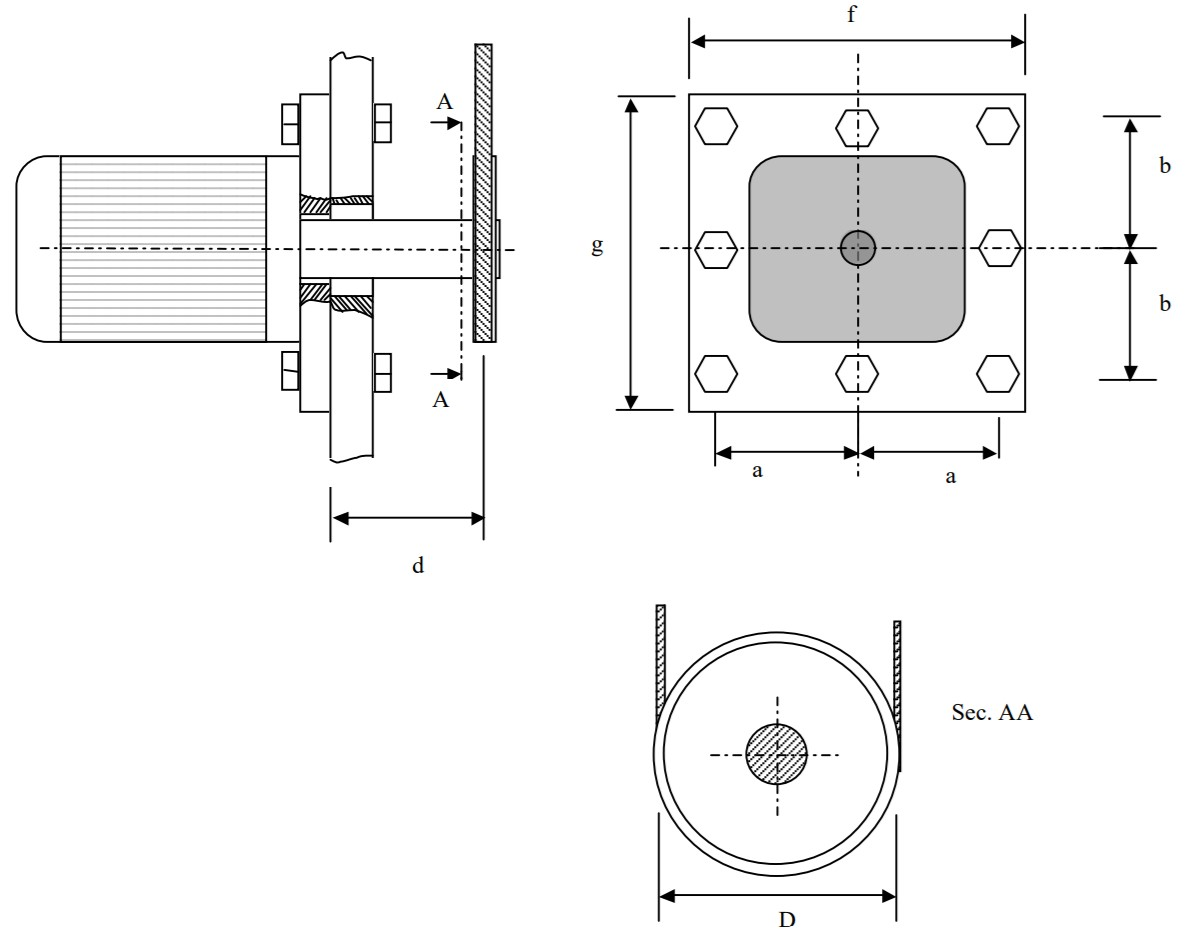
\includegraphics[width=12cm]{ex-motor}
		\caption{sketch of the bolted joint supporting an electric motor.} \label{ex:motorsketch}
	\end{figure}

	\begin{enumerate}[a)]
		\item determine the forces in both the belt sides under the most critical condition neglecting the centrifugal term;
		\item determine the bolt preload to avoid sliding between members under the hypothesis of negligible motor weight;
		\item select the bolt property class for a snug-tightened joint (no pretensioned connection) and for friction type joint with a safety factor $\phi = 1.25$.
	\end{enumerate}
	Other datas are the service factor $K_s = 1.4$, the geometrical dimensions $a = 100mm, b = 120mm, d = 140mm, D = 140mm, f=260mm, g = 300mm$, the friction coefficient belt/pulley $f_{bp} = 0.25$ and between members $f_m = 0.2$, the are of a \texttt{M5} bolt $A_{bt} = 14.2mm^2$, the UTS of the members $\sigma_{uts,m} = \sigma_{r,m} = 360MPa$ and the ordinary holes thickness $t_m = 6mm$.
	
	\paragraph{Solution}
	\begin{enumerate}[a)]
		\item the first thing is to determine the torque $T_m$ (amplified by the service factor $K_s$) determined by the motor knowing the power and the rotational speed; we in fact have that
		\[ T_m =  K_s \frac P \omega \qquad \xrightarrow{\omega = \frac{2\pi}{60} n} \quad T_m = K_s \frac{60}{2\pi} \frac{P}{n} = 142\, 603 N\cdot mm \]
		Knowing that the transmission ratio is unitary then both the drive and driven pulleys have the same diameter $D$ resulting in a contact arc $\theta_a = \pi$; neglecting the centrifugal term the tension $T_0$ on the loose side and $T_1$ on the tight can be calculated as
		\[ F_0 = \frac{T_m}{D/2} \frac{1}{e^{f_{bp} \theta_a} - 1} = 1\,707N \hspace{3cm} F_1 = \frac{T_m}{D/2} \frac{e^{f_{bp} }}{e^{f_{bp} \theta_a} - 1} = 3\,744N \]
		
		\item at this point we can compute the actions that the bolted connection must bear, and in particular we have a shear action $V = F_0 + F_1 =  5\,451N$, a torque $M_z = T_m$ and a bending moment (we consider it as applied along the $x$ axis) $M_x = (F_0+F_1) d = 763\, 225 N\cdot mm$.
		
		Starting off with the shear action, having $n_b = 8$ bolts composing the joint we have that each of them is subjected to an action $V_{i, shear} = \frac V {n_b} = 681.5N$.  		
		\begin{figure}[t]
			\centering
			\begin{subfigure}{0.48\linewidth}
				\centering 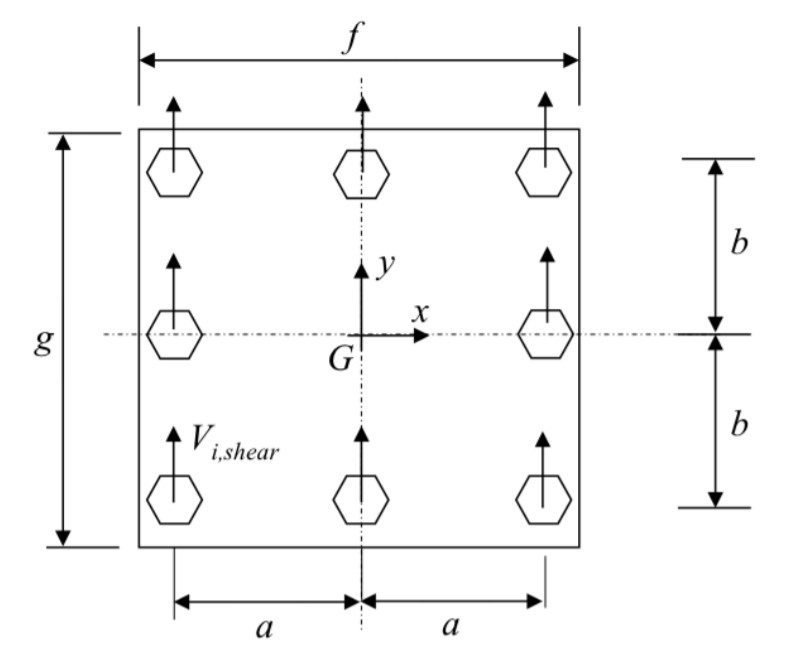
\includegraphics[width=6cm]{ex-motor-a} \caption{}
			\end{subfigure}
			\begin{subfigure}{0.48\linewidth}
				\centering 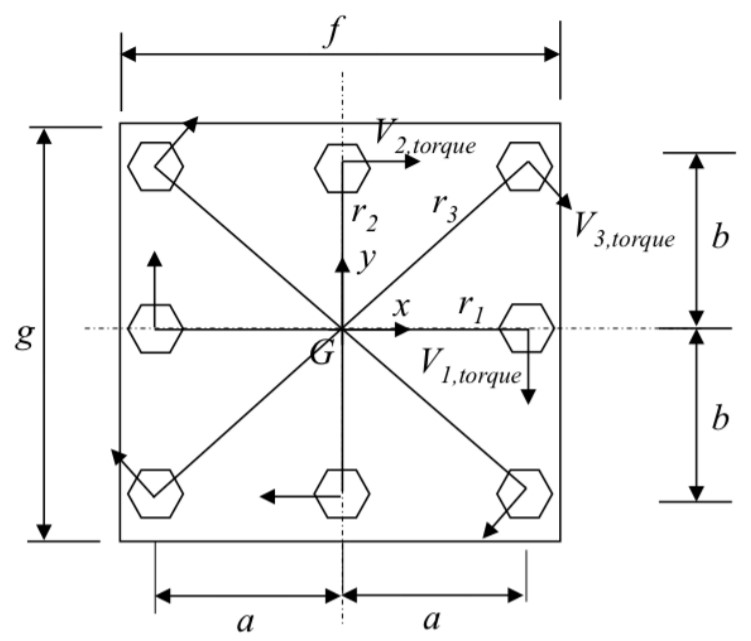
\includegraphics[width=6cm]{ex-motor-b} \caption{}
			\end{subfigure}
			\caption{distribution of the tangential action on the bolts due to shear (a) and torsion (b).} \label{fig:ex-motor-torsion}
		\end{figure}
		More complex is instead the case of the torsional load; considering the diagram in figure \ref{fig:ex-motor-torsion}.b and equation \ref{eq:slidetorsion}, knowing the three radii $r_1 = a = 100mm$, $r_2 = b = 120mm$ and $r_3 = \sqrt{a^2+b^2} = 156.2mm$ we compute the constant
		\[ C = \frac{T_m}{\sum_{i=1}^8 r_i^2} = \frac{T_m}{2r_1^2 + 2r_2^2 + 4r_3^2} = 0.974N / m \]
		that determines $V_{1,torque} = C r_1 = 97.4N$, $V_{2,torque} = C r_2 = 116.9N$ and $V_{3,torque} = C r_3 = 152.2N$. Summing vectorially the sliding action due to shear and torsion, the most critical bolts are the ones in the left conners with values
		\[ V_{B1} = V_{B3} = \sqrt{V_{3,torque}^2 + V_{3,shear}^2 + 2V_{3,torque} V_{3,shear} \cos \alpha } = 787.6N \] 	 
		where $\cos\alpha = r_1/r_3$.	To determine instead the separating action due to bending we can use the hypothesis of non-preloaded semi-rigid members where the stress state must verify $\int_A \sigma\, dA = 0$ and $\int_A\sigma y\, dA=M_x$; considering a linear distribution
		\[ \sigma = - \sigma_{max,co} \left( 1 - \frac y {y_n} \right) \]
		where the unknowns are the maximum value of the stress $\sigma_{max,co}$ and the position $y_n$ of the neutral axis, we can start an iterative process (that's checked at the end of each iteration) and assuming that all the bolts are in tension we get the system
		\[\left\{\begin{aligned}
			& - \sigma_{max,co} \frac {y_n}2 f + \sum_{i=1}^8 - \sigma_{max,co} \left( 1 - \frac{y}{y_n} \right)A_{b,i} = 0 \\
			& \sigma_{max,co} \frac{y_n}{2} f \frac{2y_n}{3} + \sum_{i=1}^8 - \sigma_{max,co} \left(1 - \frac y {y_n}\right) A_{b,i}(y_i-y_n) = M_x
		\end{aligned} \right.\]
		referred to figure \ref{ex:semirigid}.
		\begin{SCfigure}[2][bt]
			\centering 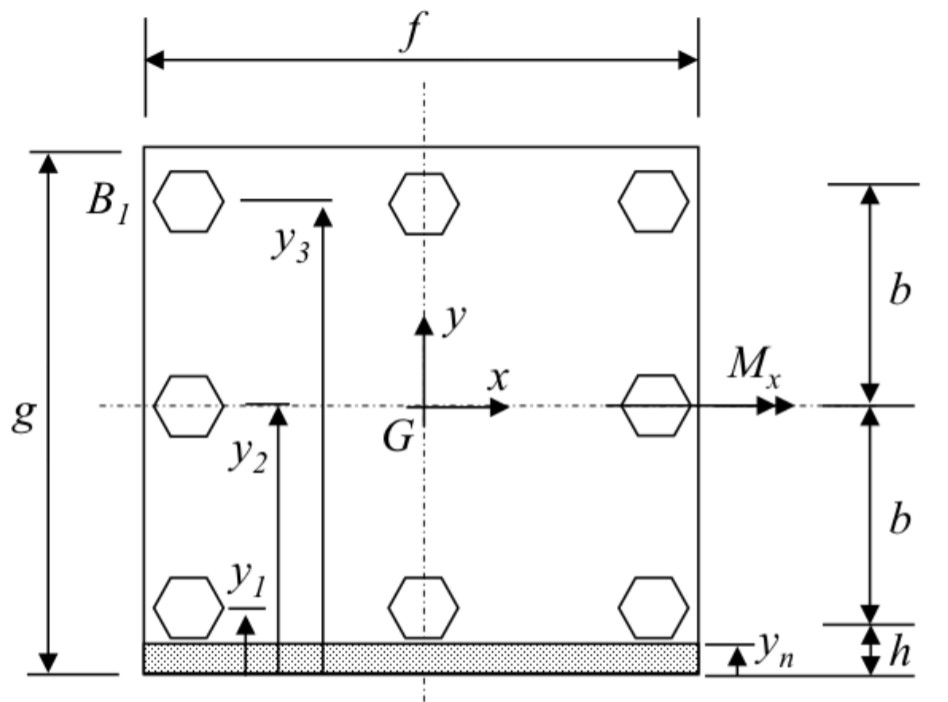
\includegraphics[width=6cm]{ex-motor-c}
			\caption{ scheme used to compute the solution of the non-preloaded semi-rigid members problem. } \label{ex:semirigid}
		\end{SCfigure}
		From the first equation we can get the position of the neutral axis, in fact by expanding the relations and collecting terms in $\sigma_{max,co}$ we determine
		\begin{align*}
			0 & = -\sigma_{max,co} \left[ \frac {y_n}2 f + 3 \left(1 - \frac{h}{y_n} \right) A_{bt} + 2 \left(1 - \frac{g/2}{y_n} \right) A_{bt}+ 3 \left(1 - \frac{g-h}{y_n} \right) A_{bt}  \right] \\
			& = -\sigma_{max,co} A_{bt} \Big[  \frac{y_n^2}{2}f + 3(y_n - h) + 2 (y_n - g/2) + 3(y_n - g+h) \Big] 
		\end{align*}
		where, determined $h = g/2-b = 30mm$, gives the solution $y_n = 11.02 mm \leq h$ verifying the assumption of all bolts in tension. Using the second equation (pre-multiplied by a factor $y_n$) we can determine the value of $\sigma_{max,co}$, solving 
		\[ M_x = \sigma_{max,co} \left[ \frac f 3 y_n^3 + A_{bt} \Big( 3(h-y_n)^2 + 2 (g/2-y_n)^2 + 3(g-h-y_n)^2 \Big)  \right]  \]
		determining $\sigma_{max,co} = 2.37MPa$. Considering that the the normal stress acting on each bolt can be computed as $\sigma_i = - \sigma_{max,co} \left(1 - \frac{y_i}{y_n}\right)$, then we have $\sigma_1 = 4.07MPa$, $\sigma_2 = 29.84MPa$ and $\sigma_3 = 55.60MPa$; the last one represent the most critical condition for the bolts that thus are subject to a separating load
		\[ N_{B1} = \sigma_3 A_{bt} = 792.3 N \]
		This action is applied on the bolt $B_1$ where also we have the highest sliding action, so that's the bolt that has to be statically verified. To compute the preload on the most critical bolt we can consider  the neutral axis as lying in the first row of bolts and only the further one (where $B_1$ is) is active, meaning that:
		\[ N_{B1}^\textrm{preload} = \frac{M_x}{\sum_{i=1}^4 \cancel{A_{bt,i}} y_i^2} y_{max} \cancel{A_{bt}} = \frac{M_x}{3 \cdot (2b^2)} 2b = \frac{M_x}{6b} = 1\,060 N \]
		
		\item Considering now the tension load estimated considering non-preloaded members about the first bolt row sw firstly need to define firstly the minimum value of $\suts$ to shear resistance. In order to use equation \ref{eq:shearresistance} it's necessary to use the nominal area $A_{nom}$ associated to the nominal diameter $d_{nom} = 5mm$ that evaluates to $\frac \pi 4 d_{nom}^2 = 19.635mm^2$; inverting equation \ref{eq:shearresistance} we have
		\[ \suts \geq \frac{V_{B1} \phi}{0.58 A_{nom}} = 86.45MPa \]
		For the tension resistance we have to consider equation \ref{eq:boltverifications} that inverted determines
		\[ \suts \geq \frac{N_{B1} \phi}{A_{bt}} = 70 MPa  \]
		According to table \ref{tab:classproperty}, a bolt with class \texttt{ISO-4014 4.6} can be used; we now need to verify both the crushing (due to the sliding actions) and the punching (due to separating loads) resistances:
		\[ V_B = 786.6 N \leq \frac{\sigma_{uts,m} d_{nom}t_m}{\phi} = 8\,640 N \hspace{2cm} N_{B1} = 792.3N \leq \frac{\pi d_\textrm{bolt,head} t_m 0.58 \sigma_{uts,m}}{\phi} =25\,189 N \]
		Having both inequalities verified then it means that the structure is statically defined.
		
		
		\textbf{MANCA LA PARTE DELLE PRELOADED BOLTED JOINTS}
		
	\end{enumerate}